\begin{frame}{$d(K^-, n K^0)"n"$  event}
  \tminipageTwo{
    \begin{figure}
      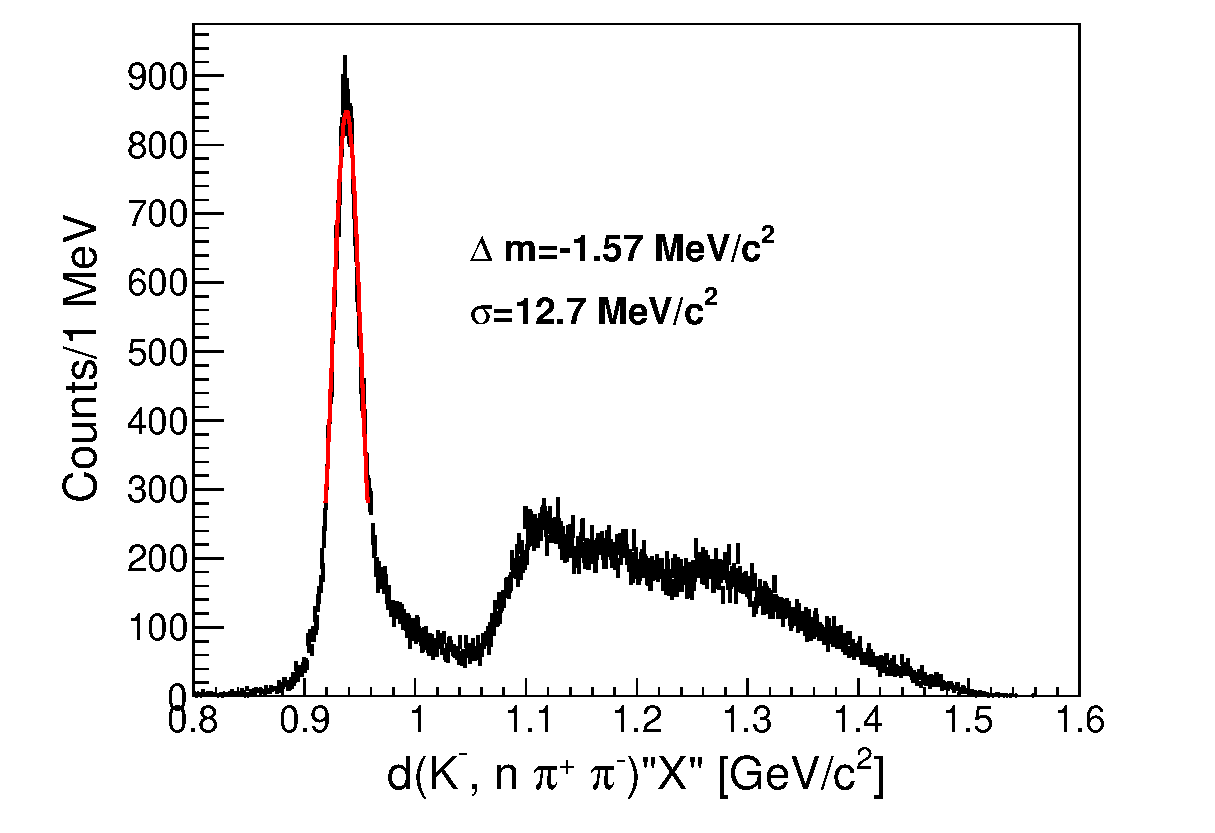
\includegraphics[width=3cm]{../pic/Run78/KN_ana_NC170_2sigma/KNpipi_MM_woFit.eps}
      \captionsetup{font=scriptsize}
      \caption{
        Event Sample : $d(K^-, n \pi^+ \pi^-)"n"$
      }
    \end{figure}
  }{
    \begin{figure} 
      \includegraphics[width=3cm]{../pic/Run78/KN_ana_NC170_2sigma/IM_pipi_select.eps}
      \captionsetup{font=scriptsize}
      \caption{
        \centering
        $K^0$ selection. \protect\linebreak
        Color plots indicates background events, \protect\linebreak
    7   which were estimated by template fittings.
%        $K^0$の選別、色線はp.\pageref{page:Fit_IM}のフィットで見積もられた。
%        バックグランドのイベントの分布を表す。
      }
    \end{figure}
  }
  \begin{tabular}{cc}
    \begin{minipage}{0.4\hsize}
      \begin{figure}
        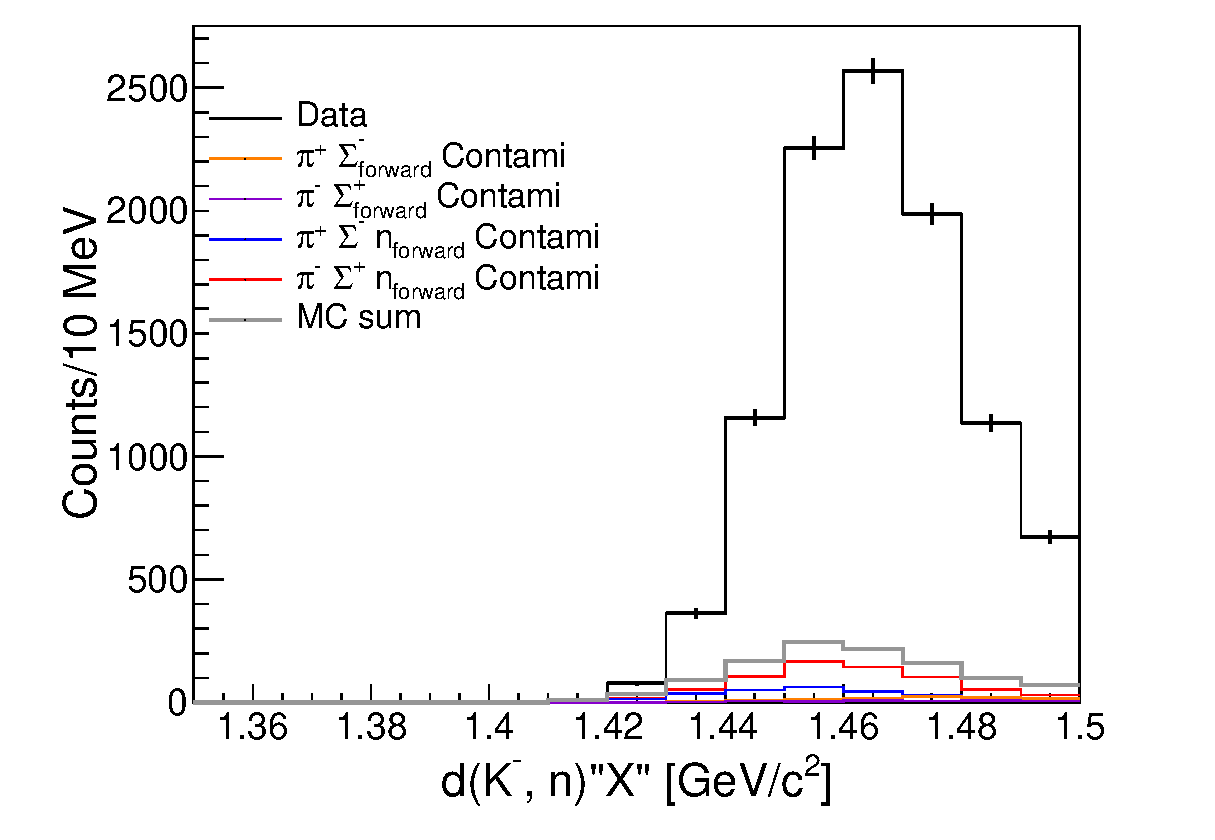
\includegraphics[width=5cm]{../pic/Run78/QE/KN_MM_wK0_tag.eps}
      \end{figure}
    \end{minipage}
    \begin{minipage}{0.6\hsize}
      \centering
      \scriptsize
      Left figure shows $d(K^-, n K^0)"n"$ events spectrum.\\
      Color plots indicate background reaction.
%      左図は上右図によって$K^0$選別されたイベント\\
%      色線は他の反応からのバックグラウンド
    \end{minipage}
  \end{tabular}
\end{frame}
